\section{Прямые на координатной плоскости задачи}
1. $\begin{tikzpicture}[scale=0.6]
\tikzset {line01/.style={line width =0.5pt}}
\tikzset{line02/.style={line width =1pt}}
\tikzset{line03/.style={dashed,line width =0.9pt}}
\filldraw [black] (0,0) circle (1pt);
\draw [->] (-2,0) -- (2,0);
\draw [->] (0,-2) -- (0,2);
\draw[line01] (-1.5,-1.7) -- (2,1);
\draw (2,0.25) node {\scriptsize $x$};
\draw (0.25,2) node {\scriptsize $y$};
\end{tikzpicture}$
На рисунке изображён график функции вида $y=kx+b.$ Для этого графика ответьте на вопросы: а) Каков знак коэффициента $k?$ б) Проходит ли график через точку $(1;b)?$\\ в) Пусть $k=\cfrac{1}{2}; b=-2.$ Проходит ли график функции через точку $(1,22;-1,38)?$\\
2. $\begin{tikzpicture}[scale=0.6]
\tikzset {line01/.style={line width =0.5pt}}
\tikzset{line02/.style={line width =1pt}}
\tikzset{line03/.style={dashed,line width =0.9pt}}
\filldraw [black] (0,0) circle (1pt);
\draw [->] (-2,0) -- (2,0);
\draw [->] (0,-2) -- (0,2);
\draw[line01] (-1.5,2) -- (2,-0.5);
\draw (2,0.25) node {\scriptsize $x$};
\draw (0.25,2) node {\scriptsize $y$};
\end{tikzpicture}$
На рисунке изображён график функции вида $y=kx+b.$ Для этого графика ответьте на вопросы: а) Каков знак коэффициента $k?$ б) Проходит ли график через точку $(-1;b)?$\\ в) Пусть $k=2; b=1.$ Проходит ли график функции через точку $(1,73;3,47)?$\\
3. Найти число $a$ такое, что точка пересечения прямых, задаваемых уравнениями \\ $y=\cfrac{1}{4}x+3a$ и $y=\cfrac{1}{2}x-a,$ имеет абсциссу 8.\\
4. Найти число $p$ такое, что точка пересечения прямых, задаваемых уравнениями \\ $y=\cfrac{1}{3}x+2p$ и $y=\cfrac{1}{2}x+p,$ имеет абсциссу 3.\\
5. Построить множество точек на координатной плоскости, координаты которых удовлетворяют уравнению $(x-5)(2y+4x-6)=0.$\\
6. Построить множество точек на координатной плоскости, координаты которых удовлетворяют уравнению $(x+4)(3y-6x+9)=0.$\\
7. При каких $a$ прямые, заданные уравнениями $x=a-3y$ и $2y=5-a-3x$ пересекаются в точке, принадлежащей прямой $y=2x+1?$\\
8. При каких $b$ прямые, заданные уравнениями $x=2y+b$ и $3y=b-1+x$ пересекаются в точке, принадлежащей прямой $y=x-8?$\\
9. При каком $k$ прямая $y=kx+4$ отсекает от осей координат в I четверти равнобедренный треугольник?\\
10. При каком $k$ прямая $y=kx+5$ отсекает от осей координат в I четверти равнобедренный треугольник?\\
11. Дана линейная функция $y=kx+1.$\\
а) Постройте график этой функции, если он проходит через точку $A(239;1196).$\\
б) При каком значении $k$ данная прямая образует вместе с осями координат прямоугольный треугольник, у которого один катет в 5 раз больше другого?\\
12. Дана линейная функция $y=ax+2.$\\
а) Постройте график этой функции, если он проходит через точку $B(79;239).$\\
б) При каком значении $a$ данная прямая образует вместе с осями координат прямоугольный треугольник, у которого один катет в 1,5 раза больше другого?\\
13. а) Постройте треугольник, ограниченный прямыми $y=\cfrac{2}{3}x+2,\ y=-\cfrac{2}{3}x-2$ и осью $OY.$\\
б) При каких значениях $b$ прямая $y=-x+b$ имеет с треугольником хотя бы одну общую точку?\\
14. а) Постройте треугольник, ограниченный прямыми $y=\cfrac{2}{3}x-2,\ y=-\cfrac{2}{3}x+2$ и осью $OY.$\\
б) При каких значениях $b$ прямая $y=-x+b$ имеет с треугольником хотя бы одну общую точку?\\
15. Известно, что прямая, заданная уравнением $y=kx+b,$ проходит через точки $A(4;-6)$ и $B(-8;-12).$ Найдите $k$ и $b,$ а также координаты точки пересечения с прямой $2x+y=2.$\\
16. Известно, что прямая, заданная уравнением $y=kx+b,$ проходит через точки $A(2;1)$ и $B(-4;10).$ Найдите $k$ и $b,$ а также координаты точки пересечения с прямой $3x-y=5.$\\
17. Постройте график функции $y=|4x-3|.$\\
18. Постройте график функции $y=4|x|-3.$\\
19. Найдите значения $k$ и $b$ функции вида $y=kx+b,$ если известно, что график функции проходит через точки $M(3;9)$ и $N(-6;-9).$ Найдите координаты точки пересечения этого графика с прямой $y=6.$\\
20. Найдите значения $k$ и $b$ функции вида $y=kx+b,$ если известно, что график функции проходит через точки $A(3;9)$ и $B(-2;-6).$ Найдите координаты точки пересечения этого графика с прямой $y=-3.$\\
21. $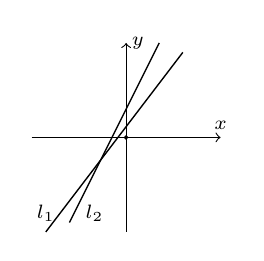
\begin{tikzpicture}[scale=0.6]
\tikzset {line01/.style={line width =0.5pt}}
\tikzset{line02/.style={line width =1pt}}
\tikzset{line03/.style={dashed,line width =0.9pt}}
\filldraw [black] (0,0) circle (1pt);
\draw [->] (-2,0) -- (2,0);
\draw [->] (0,-2) -- (0,2);
\draw[line01] (-1.7,-2) -- (1.2,1.8);
\draw[line01] (-1.2,-1.8) -- (0.7,2);
\draw (-1.7,-1.6) node {\scriptsize $l_1$};
\draw (-0.67,-1.6) node {\scriptsize $l_2$};
\draw (2,0.25) node {\scriptsize $x$};
\draw (0.25,2) node {\scriptsize $y$};
\end{tikzpicture}$ На рисунке прямая $l_1$ задана уравнением $y=k_1x+b_1,$ а прямая $l_2$ уравнением $y=k_2x+b_2.$ Сравните $k_1b_1$ и $k_2b_2.$\\
22. $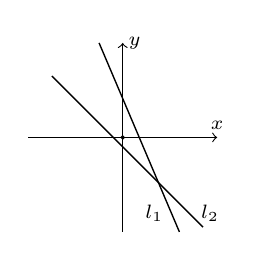
\begin{tikzpicture}[scale=0.6]
\tikzset {line01/.style={line width =0.5pt}}
\tikzset{line02/.style={line width =1pt}}
\tikzset{line03/.style={dashed,line width =0.9pt}}
\filldraw [black] (0,0) circle (1pt);
\draw [->] (-2,0) -- (2,0);
\draw [->] (0,-2) -- (0,2);
\draw[line01] (-0.5,2) -- (1.2,-2);
\draw[line01] (-1.5,1.3) -- (1.7,-1.9);
\draw (1.85,-1.6) node {\scriptsize $l_2$};
\draw (0.67,-1.6) node {\scriptsize $l_1$};
\draw (2,0.25) node {\scriptsize $x$};
\draw (0.25,2) node {\scriptsize $y$};
\end{tikzpicture}$ На рисунке прямая $l_1$ задана уравнением $y=k_1x+b_1,$ а прямая $l_2$ уравнением $y=k_2x+b_2.$ Сравните $k_1b_1$ и $k_2b_2.$\\
23. Постройте график функции $y=-3x-1$ и найдите, при каких значениях $x$ значения $y$ не больше 2.\\
24. Постройте график функции $y=-5x-4$ и найдите, при каких значениях $x$ значения $y$ не меньше 16.\\
25. Постройте множество точек $(x;y)$ на плоскости, для которых $\cfrac{(x^2-9)(y+x-1)}{x-3}=0.$\\
26. Постройте множество точек $(x;y)$ на плоскости, для которых $\cfrac{(x^2-4)(y-x+1)}{x-2}=0.$\\
27. Найдите координаты точки, через которую проходят графики функций $y=2-k-kx$ при любых значениях $k.$\\
28. Найдите координаты точки, через которую проходят графики функций $y=1-k+kx$ при любых значениях $k.$\\
29. На координатной плоскости задано множество точек $(x;y),$ причём ординаты точек вычисляются по формуле $y=3-2x.$\\
а) изобразите на координатной плоскости множество данных точек.\\
б) найдите число, квадрат которого даёт абсциссу точки $A(x;-239),$ если известно, что $A$ --- одна из точек этого множества.\\
30. На координатной плоскости задано множество точек $(x;y),$ причём ординаты точек вычисляются по формуле $y=2x-3.$\\
а) изобразите на координатной плоскости множество данных точек.\\
б) найдите число, квадрат которого даёт абсциссу точки $B(x;239),$ если известно, что $B$ --- одна из точек этого множества.\\
31. Дана функция $y=3,6x-1.$\\
а) Запишите уравнение прямой, параллельной данной и проходящей через точку $D(-0,5;8,2).$ Постройте найденную прямую.\\
б) Напишите уравнения каких-либо двух прямых, не совпадающих с осями координат, которые вместе с данной прямой ограничивают на координатной плоскости прямоугольный треугольник.\\
32. Дана функция $y=-1,5x+4.$\\
а) Запишите уравнение прямой, параллельной данной и проходящей через точку $D(7;-2,5).$ Постройте найденную прямую.\\
б) Напишите уравнения каких-либо двух прямых, не совпадающих с осями координат, которые вместе с данной прямой ограничивают на координатной плоскости прямоугольный треугольник.\\
33. Постройте график функции $y=kx+b,$ если он параллелен прямой $y=2x$ и проходит через точку $A(2;7).$ Укажите три точки, принадлежащие данному графику.\\
34. Постройте график функции $y=kx+b,$ если он параллелен прямой $y=-3x$ и проходит через точку $A(1;4).$ Укажите три точки, принадлежащие данному графику.\\
35. График линейной функции проходит через точку $A(9;-18)$ и точку пересечения прямых $y=x-7$ и $y=8x.$ Задайте функцию формулой и постройте график функции.\\
36. График линейной функции проходит через точку $A(-6;12)$ и точку пересечения прямых $y=-3x$ и $y=x+12.$ Задайте функцию формулой и постройте график функции.\\
37. Постройте график прямой $y=-6kx+3b-9,$ где числа $k$ и $b$ --- это соответственно абсцисса и ордината точки пересечения прямых $y=2x+3$ и $y=8x+7.$\\
38. Постройте график прямой $y=3kx-0,6\cdot b$ где числа $k$ и $b$ --- это соответственно абсцисса и ордината точки пересечения прямых $y=2x-4$ и $y=8x-6.$\\
39. Определите линейную функцию, если её график удовлетворяет условиям:\\
--- он параллелен графику функции $y=-3x-7$\\
--- он проходит через точку пересечения прямых, заданных уравнениями $y=-2x+2$ и $y=3x-13.$\\
40. Определите линейную функцию, если её график удовлетворяет условиям:\\
--- он параллелен графику функции $y=-2x+7$\\
--- он проходит через точку пересечения прямых, заданных уравнениями $y=2x+11$ и $y=-3x-9.$\\
41. Найдите уравнения прямых $AB$ и $CD$ и координаты точки их пересечения, если известны координаты точек: $A(3;8),\ B(12;5),\ C(4;2),\ D(2;-3).$\\
42. Найдите уравнения прямых $AB$ и $CD$ и координаты точки их пересечения, если известны координаты точек: $A(2;4),\ B(4;1),\ C(3;-4),\ D(12;2).$\\
43. Определите, лежат ли точки $A(10;-2),\ B(20;3)$ и $C(2016;1001)$ на одной прямой.\\
44. Определите, лежат ли точки $A(9;-2),\ B(18;1)$ и $C(2016;667)$ на одной прямой.\\
45. Найдите число $p,$ если известно, что точки $A\left(-\cfrac{1}{3};7
ight),\ B(3;-3)$ и $C\left(\cfrac{p-1}{2}; p
ight)$ лежат на одной прямой. Запишите уравнение этой прямой.\\
46. Найдите число $p,$ если известно, что точки $A\left(-\cfrac{1}{2};-5
ight),\ B(-4;2)$ и $C\left(\cfrac{p+2}{2}; p
ight)$ лежат на одной прямой. Запишите уравнение этой прямой.\\
47. График функции $y=kx+b$ проходит через точки $(4;-5)$ и $(k;0).$ Постройте его и найдите точку пересечения с прямой $5x-2y+17=0.$\\
48. Найдите все значения $m,$ при каждом из которых прямая $y=(2m+1)x+1-4m$ проходит через точку пересечения прямых $y=\cfrac{x}{3}-8,5$ и $y=-6x+20.$\\
49. Найдите все значения $t,$ при каждом из которых прямая $y=(2t-1)x+9,5-5t$ проходит через точку пересечения прямых $y=\cfrac{x}{3}-6,5$ и $y=-4x+26.$\\
50. Напишите уравнение прямой, параллельной прямой $y=-\cfrac{1}{2}x+11$  и проходящей через точку пересечения прямых, заданных уравнениями $y=2x-5$ и $y=-x+4.$ Постройте график заданной функции.\\
51. Напишите уравнение прямой, параллельной прямой $y=-\cfrac{1}{3}x-21$  и проходящей через точку пересечения прямых, заданных уравнениями $y=-2x+4$ и $y=\cfrac{1}{2}x+1.$ Постройте график заданной функции.\\
52. Постройте график функции $y=\cfrac{x^2}{x-1}-\cfrac{1}{x-1}.$\\
53. Рассматривается линейная функция $y=ax+b,$ найдите все значения $a$ и $b,$ при которых:\\
а) график этой функции проходит через точки $(-2;-1)$ и $(1;5).$\\
б) график этой функции не проходит через точки, произведение координат которых положительно.\\
54. Изобразите на плоскости множество точек, удовлетворяющих условию $(y-2)(x-y)=0.$\\
55. Нарисуйте множество точек, координаты которых удовлетворяют равенству $|y|=|x+1|.$\\
56. Пусть $A(2;3)$ и $B(-2;-1)$ --- две вершины квадрата. Найдите координаты двух оставшихся вершин.\\
57. Прямая $y=-0,5x+4$ пересекает ось $Ox$ в точке $B,$ а ось $Oy$ --- в точке $A.$ Считая начало координат за точку $O,$ написать уравнение прямой $BC,$ если известно, что отрезок $BA$ является медианой треугольника $CBO,$ и постройте эту прямую на координатной плоскости.\\
58. Постройте график функции $y=(x^2-4)\left(\cfrac{1}{x-2}-\cfrac{1}{x+2}
ight)-x.$\\
59. Постройте график функции $y=\cfrac{|x|}{x}\left(-\cfrac{1}{2}x+2
ight).$\\
60. Постройте график уравнения $\cfrac{(y^2-4)(y+2x-1)}{x-1}=0.$\\
61. Задайте а) графически и б) аналитически функцию, которая при $x$ таких, что $0<x<1$ принимает все значения $y$ такие, что $0\le y\le1,$ и не принимает других значений.\\
62. Найдите все значения параметра $a,$ при которых график следующей функции проходит через начало координат.
$$y=\cfrac{5a}{a-5}\cdot(x^2-1)+\cfrac{a^2}{a-5}.$$
63. Найдите все значения параметра $b,$ при которых точка графика следующей функции с абсциссой $-\cfrac{4}{3}$ лежит на оси абсцисс.
$$y=\cfrac{x-b}{3x+1}+bx.$$
64. Построить на одном чертеже графики функций $y=4x-1$ и $y=(2-0,5x): (-0,125),$
указав точки пересечения обоих графиков с осями координат и между собой, если такие точки существуют.\\
65. Пусть $A$ --- точка пересечения прямых $y=\cfrac{1}{3}x-2$ и $y=6-x.$ Напишите уравнение прямой, проходящей через точку $A$ и пересекающейся с прямой $y=-4x-3$ в точке, лежащей на оси $Oy.$ Постройте эту прямую.\\
66. График функции $f(x)=kx+3$ проходит через точку $A(-1;1).$\\
а) Постройте график этой функции. б) Найдите коэффициент $k.$\\
в) Найдите площадь треугольника, образованного этой прямой и осями координат.\\
г) Выясните, пересекается ли эта прямая с прямой $y=5x+7.$\\
67. Множество точек на координатной плоскости задано условием $a\le x \le a+6,$\\
$-a \le y \le 2a.$\\
а) Изобразите это множество при $a=3.$ б) Найдите значение $a,$ при котором указанное множество точек будет являться квадратом.\\
68. Постройте треугольник, ограниченный прямыми $y=\cfrac{1}{4}x-2;\ y=2,5$ и $y=-3x.$\\
69. Запишите уравнение прямой $ax+by=c$ (где $a,\ b,\ c$ --- целые числа), проходящей через точки $M(2;-5)$ и $N(0;-2).$\\
70. Найдите координаты точки, симметричной точке $A(3;1)$ относительно прямой $y=x+2.$\\
71. а) Упростите выражение $f(x)=\left(\cfrac{x}{x^2+2x+4}+\cfrac{x^2+8}{x^3-8}-\cfrac{1}{x-2}
ight)\cdot\left(
\cfrac{x^2}{x^2-4}-\cfrac{2}{2-x}
ight).$\\
б) Постройте график функции $y=\cfrac{1}{f(x)}.$\\
72. Даны точки $A(0;-7),\ B(3;2),\ C(1;1),\ D(-30;63).$\\
а) Напишите уравнение прямых $AB$ и $CD.$\\
б) Напишите уравнение прямой, проходящей через точку пресечения прямых $AB$ и $CD,$ пересекающей прямую $BC$ в точке, лежащей на оси абсцисс.\\
73. Даны точки $A(0;4),\ B(1;-4),\ C(-3;-2),\ D(-20;59).$\\
а) Напишите уравнение прямых $AC$ и $BD.$\\
б) Напишите уравнение прямой, проходящей через точку пресечения прямых $AC$ и $BD,$ пересекающей прямую $BC$ в точке, лежащей на оси абсцисс.\\
74. а) Постройте график функции $y=4-2x.$\\
б) Найдите расстояние от точки пересечения этого графика с осью абсцисс до точки пересечения прямых $y=x+2$ и $2x+3y-16=0.$\\
75. а) Постройте график функции $y=6-2x.$\\
б) Найдите расстояние от точки пересечения этого графика с осью абсцисс до точки пересечения прямых $y=x+3$ и $x-2y+9=0.$\\
76. Пусть точка $A$ является точкой пересечения графика функции $y=-2x+2$ с осью $OY,$ а точка $B$ --- с осью $OX.$ Напишите уравнение прямой, содержащей медиану треугольника $AOB,$ проведённую из вершины $A.$ (Точка $O$ --- начало координат)\\
77. Пусть точка $A$ является точкой пересечения графика функции $y=2x+2$ с осью $OY,$ а точка $B$ --- с осью $OX.$ Напишите уравнение прямой, содержащей медиану треугольника $AOB,$ проведённую из вершины $A.$ (Точка $O$ --- начало координат)\\
78. Прямая $y=(2a-1)x+a+3$ пересекает прямую $y=x+8$ в точке $M,$ сумма координат которой равна 6. Найдите возможные значения $a.$\\
79. При каких значений $a$ графики функций $y=2x-3,\ y=ax-a-2$ и $y=-x-6$ проходят через одну точку?\\
80. Прямая $y=(2a+1)x+a+4$ пересекает прямую $y=x+6$ в точке $A,$ сумма координат которой равна 4. Найдите возможные значения $a.$\\
81. При каких значений $a$ графики функций $y=3x-4,\ y=(a-1)x+2a-3$ и $y=-2x+1$ проходят через одну точку?\\
82. Постройте график уравнения $\cfrac{((x^2-4)^2+y^2-2y+1)(y^2-3xy+2x^2)}{xy-2y+3x-6}=0.$\\
83. Постройте график уравнения $\cfrac{((x^2-4)^2+y^2+2y+1)(y^2-4xy+3x^2)}{xy-2y+2x-4}=0.$\\
84. Дана функция $y=\cfrac{x^2-2x}{2-x}+4.$\\
а) Постройте график функции.\\
б) Какие значения принимает эта функция при положительных $x?$\\
в) Напишите уравнение прямой, проходящей через точку $(1;-1)$ и не имеющей общих точек с графиком данной функции.\\
85. Дана функция $y=\cfrac{x^2-3x}{3-x}+1.$\\
а) Постройте график функции.\\
б) Какие значения принимает эта функция при положительных $x?$\\
в) Напишите уравнение прямой, проходящей через точку $(-2;-1)$ и не имеющей общих точек с графиком данной функции.\\
86. Найдите такое число $a,$ что точка пересечения прямых $y=4x+3a$ и $y=2x+4a$ имеет ординату, равную 4.\\
87. Постройте график функции $y=\cfrac{x^2+2x}{|x|}.$\\
88. Постройте график функции $y=\cfrac{4-x^2}{x+2}-1.$ Найдите, какие целые положительные значения, меньшие 5, принимает эта функция.\\
89. \begin{figure}[ht!]
\center{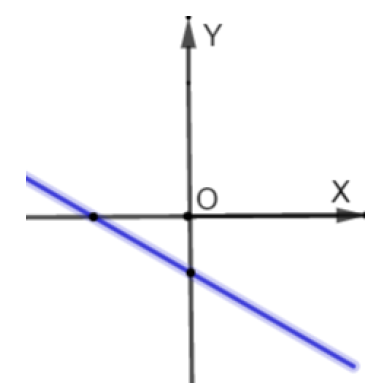
\includegraphics[scale=0.35]{gr7-89.png}}
\end{figure}\\
На рисунке изображен график функции $y=kx+d.$\\
а) Определите знак коэффициента $d.$\\
б) Проходит ли график через точку с координатами $(1; d) ?$\\
90. На координатной прямой выбраны точки $A(x + 1),\ B(x - 3)$ и $C(2x + 3).$ Найдите значения $x,$ при которых $AB = BC.$\\
91. На координатной прямой выбраны точки $A(x + 1),\ B(x - 3)$ и $C(2x + 3).$ Найдите значения $x,$ при которых $AB = AC.$\\
92. Постройте график функции: $y=\cfrac{2x^3+x^2-2x-1}{1-x^2}.$\\
93. Постройте график функции: $y=\cfrac{x^3-x^2-x+1}{1-x^2}.$\\
94. Изобразите на координатной плоскости множество точек, удовлетворяющих уравнению \\$\cfrac{(4+x(2y-x)-y^2)(x^2+y^2-2(x+y-1))}{3x+y+xy+3}=0.$\\
95. Изобразите на координатной плоскости множество точек, удовлетворяющих уравнению \\ $\cfrac{(4-x(2y+x)-y^2)}{(2x-2y+xy-4)(x^2+y^2-2(x+y-1))}=0.$

ewpage
